\documentclass{beamer}

\mode<presentation>
{
  \usetheme{default}
  \usecolortheme{default}
  \usefonttheme{default}
  \setbeamertemplate{navigation symbols}{}
  \setbeamertemplate{caption}[numbered]
  \setbeamertemplate{footline}[page number]
  \setbeamercolor{frametitle}{fg=white}
  \setbeamercolor{footline}{fg=black}
} 

\usepackage[english]{babel}
\usepackage[utf8x]{inputenc}
\usepackage{tikz}
\usepackage{listings}
\usepackage{courier}
\usepackage{array}
\usepackage{bold-extra}
\usepackage{minted}
\usepackage{transparent}

\xdefinecolor{darkblue}{rgb}{0.1,0.1,0.7}
\xdefinecolor{darkgreen}{rgb}{0,0.5,0}
\xdefinecolor{darkgrey}{rgb}{0.35,0.35,0.35}
\xdefinecolor{darkorange}{rgb}{0.8,0.5,0}
\xdefinecolor{darkred}{rgb}{0.7,0,0}
\xdefinecolor{dianablue}{rgb}{0.18,0.24,0.31}
\definecolor{commentgreen}{rgb}{0,0.6,0}
\definecolor{stringmauve}{rgb}{0.58,0,0.82}

\lstset{ %
  backgroundcolor=\color{white},      % choose the background color
  basicstyle=\ttfamily\small,         % size of fonts used for the code
  breaklines=true,                    % automatic line breaking only at whitespace
  captionpos=b,                       % sets the caption-position to bottom
  commentstyle=\color{commentgreen},  % comment style
  escapeinside={\%*}{*)},             % if you want to add LaTeX within your code
  keywordstyle=\color{blue},          % keyword style
  stringstyle=\color{stringmauve},    % string literal style
  showstringspaces=false,
  showlines=true
}

\lstdefinelanguage{scala}{
  morekeywords={abstract,case,catch,class,def,%
    do,else,extends,false,final,finally,%
    for,if,implicit,import,match,mixin,%
    new,null,object,override,package,%
    private,protected,requires,return,sealed,%
    super,this,throw,trait,true,try,%
    type,val,var,while,with,yield},
  otherkeywords={=>,<-,<\%,<:,>:,\#,@},
  sensitive=true,
  morecomment=[l]{//},
  morecomment=[n]{/*}{*/},
  morestring=[b]",
  morestring=[b]',
  morestring=[b]"""
}

\title[2017-05-11-dshep]{\bf \LARGE Data plumbing: \\ moving data across frameworks}
\author{Jim Pivarski}
\institute{Princeton University -- DIANA}
\date{May 11, 2017}

\begin{document}

\logo{\pgfputat{\pgfxy(0.11, 8)}{\pgfbox[right,base]{\tikz{\filldraw[fill=dianablue, draw=none] (0 cm, 0 cm) rectangle (50 cm, 1 cm);}}}\pgfputat{\pgfxy(0.11, -0.6)}{\pgfbox[right,base]{\tikz{\filldraw[fill=dianablue, draw=none] (0 cm, 0 cm) rectangle (50 cm, 1 cm);}
\includegraphics[height=0.99 cm]{diana-hep-logo.png}\tikz{\filldraw[fill=dianablue, draw=none] (0 cm, 0 cm) rectangle (4.9 cm, 1 cm);}}}}

\usebackgroundtemplate{{\transparent{0.15}
\includegraphics[width=\paperwidth,height=\paperheight]{plumbing.jpg}}}

\begin{frame}
  \titlepage
\end{frame}

\usebackgroundtemplate{}

\logo{\pgfputat{\pgfxy(0.11, 8)}{\pgfbox[right,base]{\tikz{\filldraw[fill=dianablue, draw=none] (0 cm, 0 cm) rectangle (50 cm, 1 cm);}
\includegraphics[height=1 cm]{diana-hep-logo.png}}}}

% Uncomment these lines for an automatically generated outline.
%\begin{frame}{Outline}
%  \tableofcontents
%\end{frame}

%%%%%%%%%%%%%%%%%%%%%%%%%%%%%%%%%%%%%%%%%%%%%%%%%%%%%%%

\begin{frame}{Why worry about moving data?}
We're all here because we think that HEP can benefit from machine learning techniques.

\vfill
\uncover<2->{The most advanced techniques are being developed \mbox{outside of HEP,\hspace{-1 cm}} using (what are becoming) industry standard tools.}

\vfill
\uncover<3->{\textcolor{darkblue}{Problem:} our HEP protocols and formats won't work with them without some modification or export.}

\vfill
\uncover<4->{\textcolor{darkblue}{This talk is about solutions to that problem.}}
\end{frame}

\begin{frame}{}

\only<1>{\mbox{\hspace{-1 cm}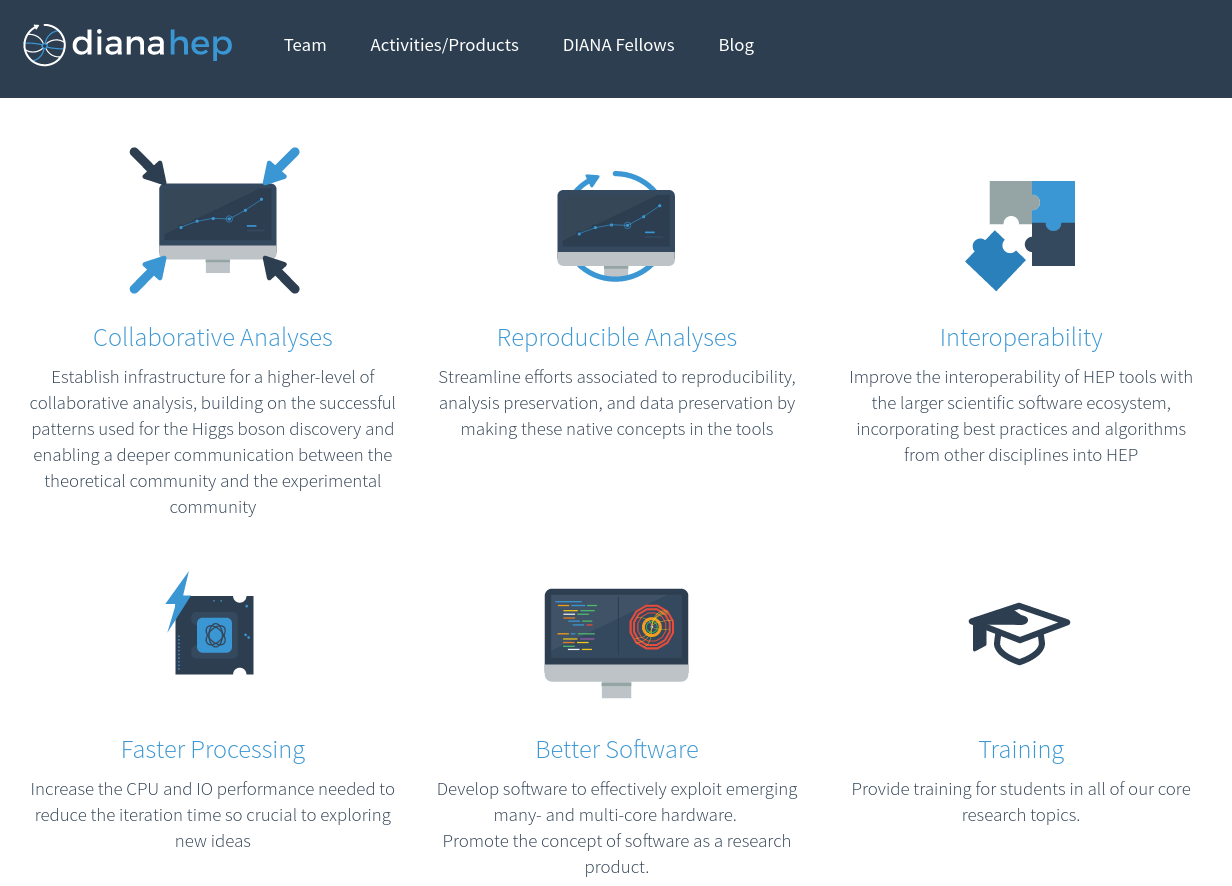
\includegraphics[width=1.2\linewidth]{diana-hep.png}}}
\only<2>{\mbox{\hspace{-1 cm}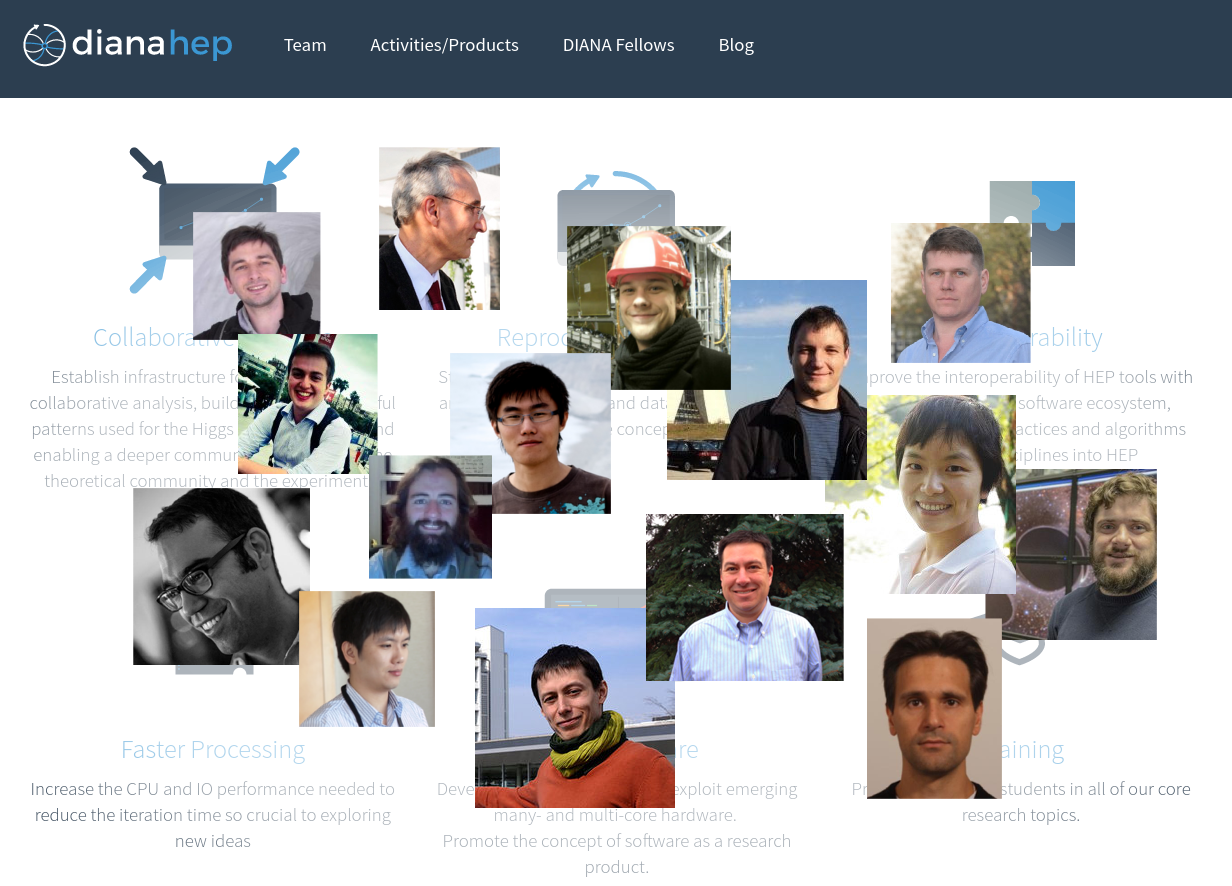
\includegraphics[width=1.2\linewidth]{diana-hep2.png}}}

\end{frame}

\begin{frame}{Goals of this talk}
\Large
\begin{itemize}\setlength{\itemsep}{0.5 cm}
\item \textcolor{darkblue}{make \underline{you} aware of what's possible}
\item \textcolor{darkblue}{introduce some software tools}
\item \textcolor{darkblue}{invite you to tell \underline{me} what's needed.}
\end{itemize}
\end{frame}

\begin{frame}{}
\begin{center}
\LARGE \textcolor{darkblue}{ROOT and Numpy}
\end{center}
\end{frame}

\begin{frame}[frame]{root\_numpy}
\vfill
\begin{columns}[t]
\column{0.5\linewidth}
\textcolor{darkblue}{ROOT} is the standard for HEP data storage and processing.
\column{0.5\linewidth}
\textcolor{darkblue}{Numpy} is the standard for the scientific Python ecosystem: {\small SciPy,} {\small Scikit-Learn,} {\footnotesize TensorFlow,} {\footnotesize Keras,} {\scriptsize PyTorch,} {\scriptsize DyNet,} {\tiny MinPy,} {\tiny MXNet\ldots}
\end{columns}

\vfill
\begin{uncoverenv}<2->

\includegraphics[height=2.5 cm]{scikit-hep_logo_800.png}

\vspace{-2.5 cm}
\hfill \begin{minipage}{0.7\linewidth}
{\bf root\_numpy} from Scikit-HEP provides high-level translation to/from ROOT TTrees and Numpy arrays.

\vspace{0.5 cm}
\textcolor{blue}{\underline{\url{http://scikit-hep.org/root_numpy/}}}
\end{minipage}
\end{uncoverenv}
\end{frame}

\begin{frame}[fragile]{Examples}
\footnotesize
\begin{minted}{python}
import root_numpy

# get an array from a ROOT file named by string
filename = root_numpy.testdata.get_filepath("test.root")
array1 = root_numpy.root2array(filename, "tree")

# or get an array from a PyROOT TFile/TTree
import ROOT
rootfile = ROOT.TFile(filename)
roottree = rootfile.Get("tree")
array2 = root_numpy.tree2array(roottree)
\end{minted}

\vspace{0.5 cm}
\begin{uncoverenv}<2->
{\normalsize Use {\tt TTree::Draw} syntax to transform branches and cut events.}

\begin{minted}{python}
array3 = root_numpy.tree2array(roottree,
    branches=["x", "y", "sqrt(y)", "TMath::Landau(x)"],
    selection="z > 0")
\end{minted}
\end{uncoverenv}
\end{frame}

\begin{frame}{Worth noting\ldots}
\vspace{0.25 cm}
\begin{itemize}\setlength{\itemsep}{0.5 cm}
\item Although root\_numpy currently loads whole branches into memory at once, it's possible to extend to {\it streaming} C++ APIs (hint: TensorFlow Queues).

\item There are other extensions ``out there,'' such as this one:
\begin{center}
\textcolor{blue}{\underline{\url{https://github.com/ibab/root_pandas}}}
\end{center}

\item Scikit-HEP is a metapackage (developers below) to try to make things like this easier to find.

\footnotesize
\vspace{0.25 cm}
Noel Dawe (University of Melbourne), Vanya Belyaev (ITEP), Sasha Mazurov (University of Birmingham), Eduardo Rodrigues (University of Cincinnati), David Lange (Princeton University), and myself.
\end{itemize}
\end{frame}

\begin{frame}{}
\begin{center}
\LARGE \textcolor{darkblue}{direct to Numpy}
\end{center}
\end{frame}

\begin{frame}{Skip the middleman}
\vspace{0.25 cm}
root\_numpy is great if you have a lot of ROOT files and need to analyze them in Python.

\vspace{0.25 cm}
\uncover<2->{But if you don't already have the ROOT files, generating and then converting them is awkward, especially if the dataset is large.}

\begin{uncoverenv}<3->
\vspace{0.25 cm}
\begin{block}{Fortunately, the Numpy format is extremely simple.}
\begin{itemize}\setlength{\itemsep}{0.5 cm}
\item<4-> a Numpy array is a plain C array interpreted by metadata {\small (data type,} {\footnotesize number of elements,} {\scriptsize endianness,} {\tiny C vs.\ Fortran-style stride\ldots)}
\begin{itemize}
\item you can wrap any region of memory as a Numpy array
\end{itemize}

\item<5-> a Numpy file is a literal copy of the array with a header
\begin{itemize}
\item you can write Numpy files with minimal code
\end{itemize}

\end{itemize}
\end{block}
\end{uncoverenv}
\end{frame}

\begin{frame}[fragile]{Examples of wrapping arrays}
\vspace{0.25 cm}
If PyROOT gives you an {\tt array.array}, wrap it like this:

\small
\begin{minted}{python}
    import numpy
    numpy_array = numpy.frombuffer(array_from_root)
\end{minted}

\normalsize
Now it has Numpy powers.

\begin{uncoverenv}<2->
\vspace{0.25 cm}
As long as you perform in-place operations, like

\small
\begin{minted}{python}
    # overwrite all elements x with sin(x)
    numpy.sin(numpy_array, numpy_array)
    # set all values to 3.14
    numpy_array[:] = 3.14
\end{minted}

\normalsize
it will modify the same memory that ROOT is looking at.
\end{uncoverenv}

\begin{uncoverenv}<3->
\vspace{0.25 cm}
\textcolor{darkblue}{With great power comes great responsibility:} if ROOT deletes this array and you continue to modify it, you will corrupt memory, causing a segmentation fault {\it at best.}
\end{uncoverenv}
\end{frame}

\begin{frame}[fragile]{Examples of wrapping arrays}
\vspace{0.25 cm}
You can split a Python script into parallel processes using its builtin {\tt multiprocessing} module. These processes can share a block of memory, which you can wrap with Numpy.

\vspace{0.25 cm}
See \textcolor{blue}{\underline{\url{https://goo.gl/NPwcSL}}} for an example.

\vfill
\begin{uncoverenv}<2->
\textcolor{darkblue}{Another possible use:} point Python and a C++ framework (e.g.\ Athena or CMSSW) to the same shared memory to transfer data between them at runtime.

\vspace{0.25 cm}
Also known as a ``common block.'' \hspace{0.25 cm}{\tt :)}

\vspace{0.25 cm}
\textcolor{gray}{(A good implementation would be wrapped in a thread-safe, type-safe API, of course!)}
\end{uncoverenv}
\end{frame}

\begin{frame}[fragile]{Examples of wrapping arrays}
\vspace{0.5 cm}
\hfill 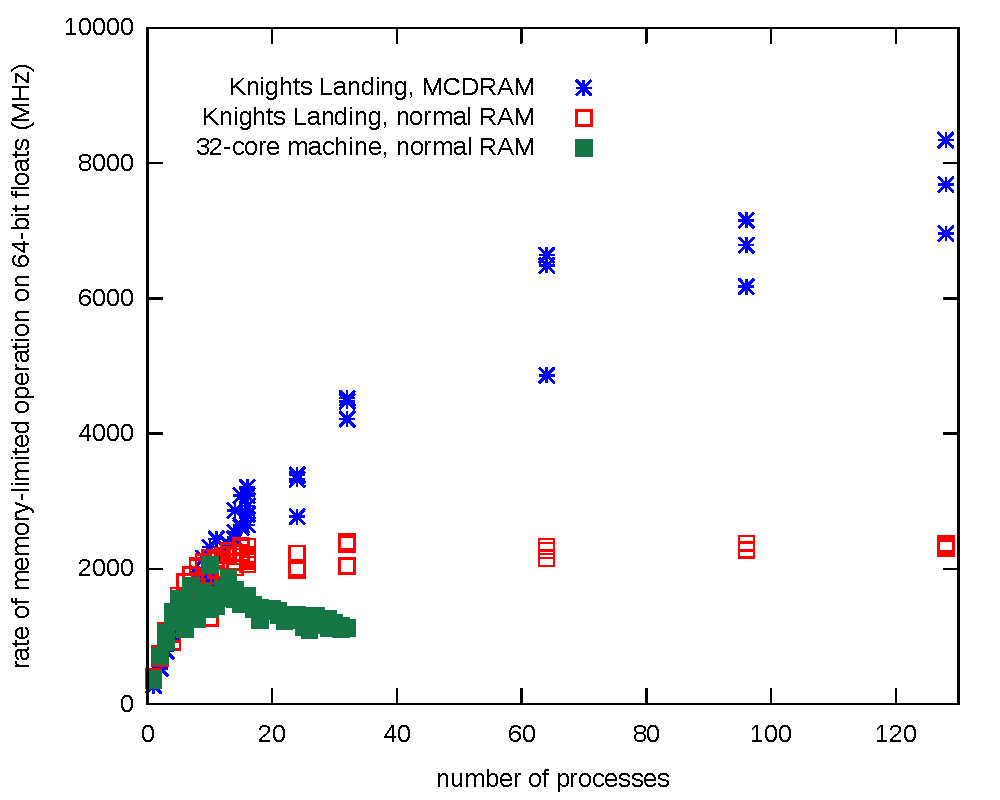
\includegraphics[height=3.5 cm]{knl-scaling.pdf}

\vspace{-3.5 cm}
Even use non-standard allocators \\ (this one allocates memory on \\ Knight's Landing MCDRAM).

\vspace{0.25 cm}
\scriptsize
\begin{minted}{python}
import ctypes
import numpy

ZILLION = 1000000

libnuma = ctypes.cdll.LoadLibrary("libnuma.so")
libnuma.numa_alloc_local.restype = ctypes.POINTER(ctypes.c_double)
ptr = libnuma.numa_alloc_local(ctypes.c_size_t(ZILLION))

ptr.__array_interface__ =
    {"version": 3,
     "typestr": numpy.ctypeslib._dtype(type(ptr.contents)).str,
     "data": (ctypes.addressof(ptr.contents), False),
     "shape": (ZILLION,)}

asarray = numpy.array(ptr, copy=False)
\end{minted}
\end{frame}

\begin{frame}[fragile]{Writing Numpy files is easy, too}
\begin{center}
\textcolor{blue}{\underline{\url{https://github.com/diana-hep/c2numpy}}}
\end{center}

Pure-header C library: drop it in and write Numpy files.

\vspace{0.25 cm}
\scriptsize
\begin{minted}{c++}
#include "c2numpy.h"

c2numpy_init(&writer, "output/tracks", 1000);
c2numpy_addcolumn(&writer, "pt", C2NUMPY_FLOAT64);
c2numpy_addcolumn(&writer, "eta", C2NUMPY_FLOAT64);
c2numpy_addcolumn(&writer, "phi", C2NUMPY_FLOAT64);
c2numpy_addcolumn(&writer, "dxy", C2NUMPY_FLOAT64);
c2numpy_addcolumn(&writer, "dz", C2NUMPY_FLOAT64);

...

for (auto track = tracks->cbegin();
     track != tracks->end();
     ++track) {
  c2numpy_float64(&writer, track->pt());
  c2numpy_float64(&writer, track->eta());
  c2numpy_float64(&writer, track->phi());
  c2numpy_float64(&writer, track->dxy());
  c2numpy_float64(&writer, track->dz());
}
\end{minted}
\end{frame}

\begin{frame}{}
\begin{center}
\LARGE \textcolor{darkblue}{industry standard formats}

\vspace{0.25 cm}
\textcolor{darkblue}{\Large Avro/Thrift/ProtoBuf, Parquet/Feather, Arrow}
\end{center}
\end{frame}

\begin{frame}{What about nested structure?}
\vspace{0.5 cm}
Numpy isn't appropriate (efficient) for anything but flat-flat ntuples: strictly columns of numbers, no {\tt\small std::vector<double>}!

\vfill
\begin{uncoverenv}<2->
ROOT pioneered efficient storage of nested, hierarchical data with built-in schema (TTrees), but today there are other options:

\begin{center}
\begin{tabular}{l l}
\textcolor{darkblue}{row-wise (``unsplit'')} & Avro, Thrift, ProtoBuf \\
\textcolor{darkblue}{columnar (``split'')} & Parquet, Feather \\
\textcolor{darkblue}{in-memory} & Arrow
\end{tabular}
\end{center}
\end{uncoverenv}
\end{frame}

\begin{frame}{Abstract type systems}
\vspace{0.25 cm}
All of these formats are interconvertable and accessible in dozens of programming languages because they're all based on roughly the same abstract type systems.

\vspace{0.25 cm}
\textcolor{darkblue}{Data types are}
\begin{description}
\item[null:] only one possible value, usually not written explicitly
\item[boolean:] true or false
\item[integer:] whole numbers
\item[float:] floating-point numbers (usually with specified precision)
\item[string:] usually UTF-8
\item[list:] arbitrary length collections of the above
\item[record:] structs whose fields are any of the above
\item[union:] one type {\it or} another type (tagged)
\end{description}
\textcolor{darkblue}{but no pointers/TRefs or class methods (functions).}
\end{frame}

\begin{frame}{Automated conversion}

\begin{center}
\textcolor{blue}{\underline{\url{https://github.com/diana-hep/rootconverter}}}
\end{center}

is an {\it unmaintained} software package that converted ROOT files, including any nested classes, into Avro format. It mapped ROOT's {\tt\small TStreamerInfo} onto the corresponding abstract data types.

\vfill
It could be resurrected or repurposed if there's a need: the point is that this is {\it possible.}
\end{frame}

\begin{frame}{}
\begin{center}
\LARGE \textcolor{darkblue}{Spark and the JVM}
\end{center}
\end{frame}

\begin{frame}{Reading ROOT files in Spark}
This was developed as part of a project to perform a CMS analysis in Apache Spark.

\begin{center}
\textcolor{blue}{\underline{\url{https://cms-big-data.github.io/}}}
\end{center}

Last year, we converted all data from ROOT to Avro because Spark recognizes the Avro format (previous page).

\vfill
\textcolor{darkblue}{This year, we're using a pure Java implementation of the ROOT format to load data directly into Spark.}
\end{frame}

\begin{frame}{}

\only<1-2>{{\mbox{\hspace{-1 cm}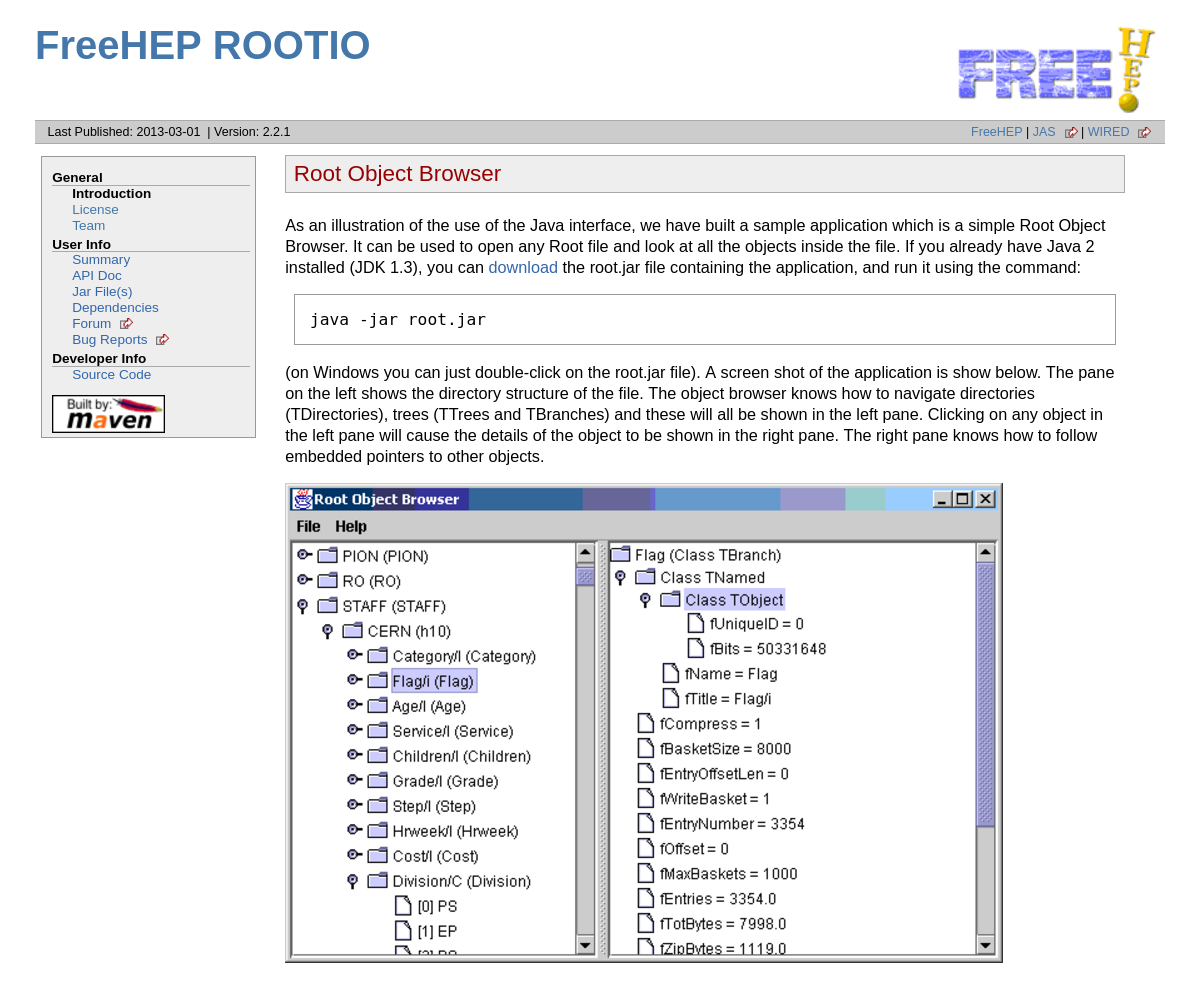
\includegraphics[width=1.2\linewidth]{rootio-screenshot.png}}}}
\only<3-4>{{\mbox{\hspace{-1 cm}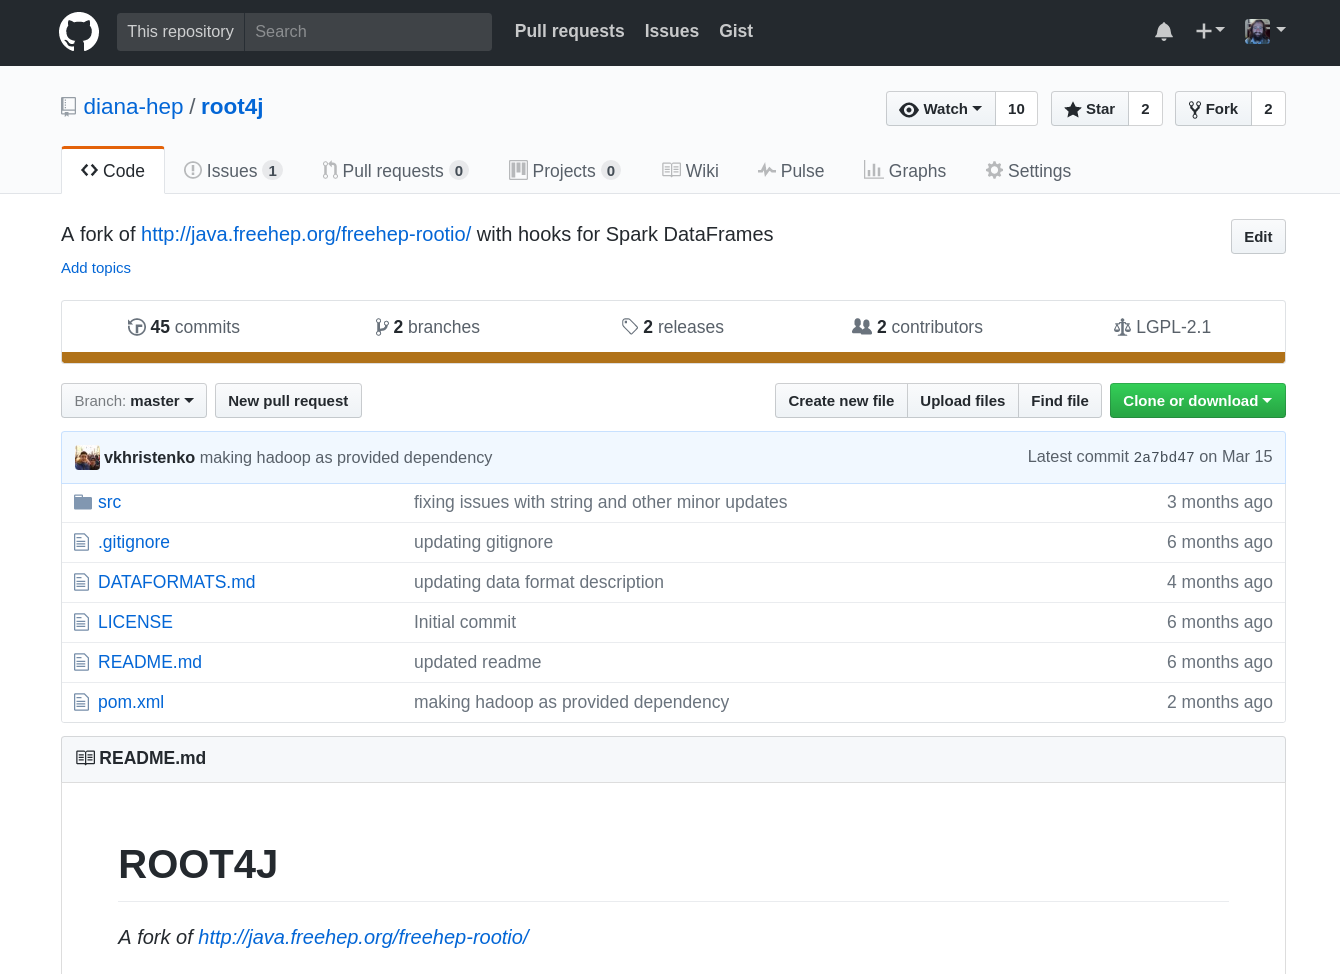
\includegraphics[width=1.2\linewidth]{root4j.png}}}}

\begin{onlyenv}<2>
\vspace{-6.2 cm}\hfill\begin{minipage}{3 cm}
\begin{center}
\mbox{\begin{minipage}{2.3 cm}
\centering 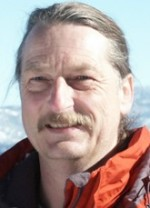
\includegraphics[width=2 cm]{tonyJohnson_new.jpg}

\centering Tony Johnson

\centering SLAC
\end{minipage}\hspace{-3.2 cm}}
\end{center}
\end{minipage}\hspace{1 cm}\vspace{3.5 cm}
\end{onlyenv}
\begin{onlyenv}<4>
\vspace{-3.5 cm}\hfill\begin{minipage}{3 cm}
\begin{center}
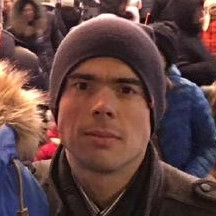
\includegraphics[width=2 cm]{viktor.jpg}

Viktor Khristenko

{\small University of Iowa}
\end{center}
\end{minipage}\hspace{1 cm}\vspace{3.5 cm}
\end{onlyenv}

\end{frame}

\begin{frame}[fragile]{Example session (\only<1>{Spark}\only<2>{PySpark})}
\vspace{0.5 cm}
Launch Spark with packages from Maven Central.
\small
\begin{onlyenv}<1>
\begin{minted}{bash}
spark-shell --packages \
    org.diana-hep:spark-root_2.11:0.1.11
\end{minted}
\end{onlyenv}
\begin{onlyenv}<2>
\begin{minted}{bash}
pyspark --packages \
    org.diana-hep:spark-root_2.11:0.1.11
\end{minted}
\end{onlyenv}

\normalsize
Read ROOT file like any other format for a DataFrame.

\small
\begin{onlyenv}<1>
\begin{minted}{scala}
import org.dianahep.sparkroot._
val df = spark.sqlContext.read.root(
             "hdfs://path/to/files/*.root")
\end{minted}
\end{onlyenv}
\begin{onlyenv}<2>
\begin{minted}{python}
df = sqlContext.read \
       .format("org.dianahep.sparkroot") \
       .load("hdfs://path/to/files/*.root")
\end{minted}
\end{onlyenv}

\begin{verbatim}
df.printSchema()
root
 |-- met: float (nullable = false)
 |-- muons: array (nullable = false)
 |    |-- element: struct (containsNull = false)
 |    |    |-- pt: float (nullable = false)
 |    |    |-- eta: float (nullable = false)
 |    |    |-- phi: float (nullable = false)
 |-- jets: array (nullable = false)
\end{verbatim}
\end{frame}

\begin{frame}[fragile]{Example session (\only<1>{Spark}\only<2>{PySpark})}
\small
\begin{verbatim}
df.show()
+---------+--------------------+--------------------+
|      met|               muons|                jets|
+---------+--------------------+--------------------+
| 55.59374|[[28.07075,-1.331...|[[194.19714,-2.65...|
|39.440292|                  []|[[93.64958,-0.273...|
|2.1817229|[[5.523367,-0.375...|[[96.09923,0.7058...|
|  80.5822|[[48.910114,-0.17...|[[165.2686,0.2623...|
| 84.43806|                  []|[[51.87823,1.6442...|
| 84.63146|[[33.84279,-0.062...|[[137.74776,-0.45...|
| 393.8167|[[25.402626,-0.66...|[[481.8268,-1.115...|
|  75.0873|                  []|[[144.62373,-2.21...|
|2.6512942|[[6.851382,2.3145...|[[72.08256,-1.713...|
|36.753353|                  []|[[72.7172,-1.3265...|
+---------+--------------------+--------------------+
only showing top 10 rows
\end{verbatim}
\end{frame}

\begin{frame}[fragile]{Example session (\only<1>{Spark}\only<2>{PySpark})}
\vspace{0.25 cm}
(This is from a real CMS analysis.)

\begin{onlyenv}<1>
\small
\begin{minted}{scala}
// Bring dollar-sign notation into scope.
import spark.sqlContext.implicits._

// Compute event weight with columns and constants.
df.select(($"lumi"*xsec/nGen) * $"LHE_weight"(309))
  .show()

// Pre-defined function (notation's a little weird).
val isGoodEvent = (
    ($"evtHasGoodVtx" === 1) &&
    ($"evtHasTrg" === 1)     &&
    ($"tkmet" >= 25.0)       &&
    ($"Mu_pt" >= 30.0)       &&
    ($"W_mt" >= 30.0))

// Use it.
println("%d events pass".format(
                    df.where(isGoodEvent).count()))
\end{minted}
\end{onlyenv}

\begin{onlyenv}<2>
\small
\begin{minted}{python}
# Python trick: make columns Python variables.
for name in df.schema.names:
    exec("{0} = df['{0}']".format(name))

# Look at a few event weights.
df.select((lumi*xsec/nGen) * LHE_weight[309]).show()

# Pre-defined function (notation's a little different).
isGoodEvent = (
    (evtHasGoodVtx == 1) &
    (evtHasTrg == 1)     &
    (tkmet >= 25.0)      &
    (Mu_pt >= 30.0)      &
    (W_mt >= 30.0))

# Use it.
print "{} events pass".format(
                  df.where(isGoodEvent).count())
\end{minted}
\end{onlyenv}
\end{frame}

\begin{frame}[fragile]{Example session (\only<1>{Spark}\only<2->{PySpark})}
\vspace{0.25 cm}
\small
\begin{onlyenv}<1>
\begin{minted}{bash}
spark-shell --packages \
    org.diana-hep:spark-root_2.11:0.1.11, \
    org.diana-hep:histogrammar_2.11:1.0.4
\end{minted}
\end{onlyenv}
\begin{onlyenv}<2->
\begin{minted}{bash}
pyspark --packages \
    org.diana-hep:spark-root_2.11:0.1.11, \
    org.diana-hep:histogrammar_2.11:1.0.4
\end{minted}
\end{onlyenv}
\small
\begin{onlyenv}<1>
\begin{minted}{scala}
// Use Histogrammar to make histograms.
import org.dianahep.histogrammar._
import org.dianahep.histogrammar.sparksql._
import org.dianahep.histogrammar.bokeh._

// Define histogram functions with SparkSQL Columns.
val h = df.Label(
         "muon pt" -> Bin(100, 0.0, 50.0, $"Mu_pt"),
         "W mt" -> Bin(100, 0.0, 120.0, $"W_mt"))

// Plot the histograms with Bokeh.
val bokehhist = h.get("muon pt").bokeh()
plot(bokehhist)
val bokehhist2 = h.get("W mt").bokeh()
plot(bokehhist2)
\end{minted}
\end{onlyenv}

\begin{onlyenv}<2->
\begin{minted}{python}
# Use Histogrammar to make histograms.
from histogrammar import *
import histogrammar.sparksql
histogrammar.sparksql.addMethods(df)

# Define histogram functions with SparkSQL Columns.
h = df.Label(
      muon_pt = Bin(100, 0.0, 50.0, Mu_pt),
      W_mt = Bin(100, 0.0, 120.0, W_mt))

# Plot the histograms with PyROOT.
roothist = h.get("muon_pt").plot.root("muon pt")
roothist.Draw()
roothist2 = h.get("W_mt").plot.root("W mt")
roothist2.Draw()
\end{minted}
\end{onlyenv}

\vspace{-3.1 cm}
\begin{uncoverenv}<3>
\mbox{ } \hfill 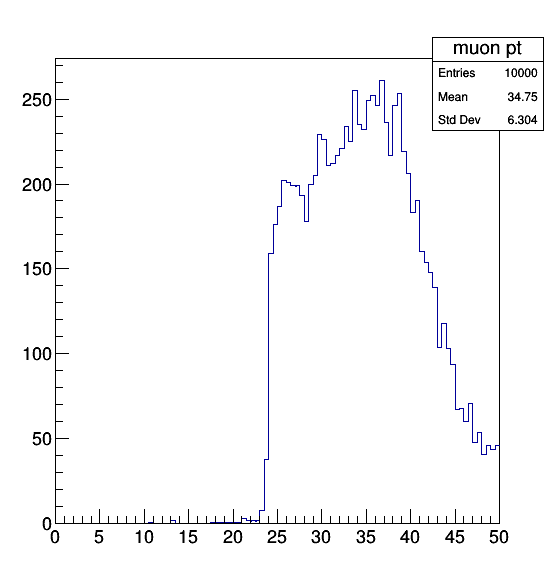
\includegraphics[width=3 cm]{muonpt.png}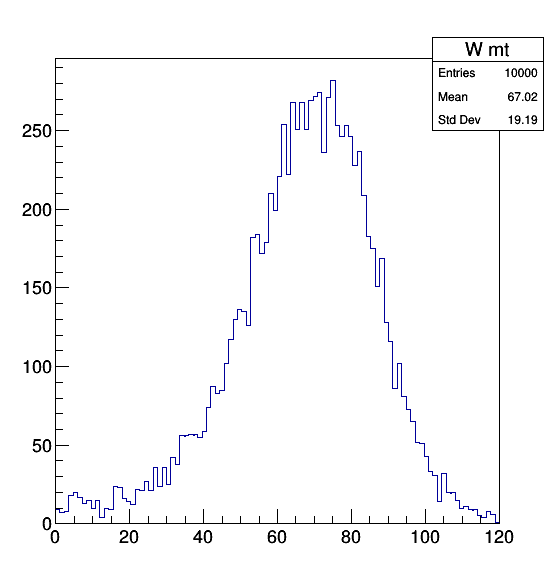
\includegraphics[width=3 cm]{wmt.png}
\end{uncoverenv}
\end{frame}

\begin{frame}{Not just Spark}
\vspace{0.5 cm}
root4j (ROOT reader) is separate from spark-root.

\vfill
\textcolor{darkblue}{root4j opens the door to {\it all} the Java-based big data tools.}

\vfill
As far as I'm aware, it is one of only five ROOT TTree readers:
\begin{center}
\renewcommand{\arraystretch}{1.2}
\begin{tabular}{r | l}
standard ROOT & C++ \\
JsRoot        & JavaScript\hspace{0.75 cm} \\
root4j        & Java \\
RIO in GEANT  & C++ \\
go-hep        & go
\end{tabular}
\end{center}
\end{frame}

\begin{frame}{Conclusing remarks}
\vfill
\vfill
\textcolor{darkblue}{Perhaps you saw something here and thought,}
\begin{itemize}
\item ``I can use that to avoid my awful work-around!'' \textcolor{darkblue}{or}
\item ``I didn't think that was possible! Now I can do something I wouldn't have considered before,'' \textcolor{darkblue}{or}
\item ``What I want to do is possible, but it will take some work.''
\end{itemize}

\vfill
\begin{uncoverenv}<2->
If so, contact me and I may be able to help. I know or am the author of several of these packages, and can help you get started if you need to develop something new.

\vfill
\begin{center}
\textcolor{darkblue}{\tt pivarski@fnal.gov}
\end{center}
\end{uncoverenv}
\end{frame}

\end{document}
